
\section{shells}

\subsection{shells, the concept}

\begin{frame}{shell}
\begin{itemize}
    \item allow user (= person at keyboard) to run applications
    \item user's wrapper around process-management functions
\end{itemize}
\end{frame}

\begin{frame}{aside: shell forms}
\begin{itemize}
    \item POSIX: command line you have used before
        \vspace{.5cm}
    \item also: graphical shells
        \begin{itemize}
        \item e.g. OS X Finder, Windows explorer
        \end{itemize}
    \item other types of command lines?
    \item completely different interfaces?
\end{itemize}
\end{frame}



\subsection{I/O redirection: syntax, method preview}

\againframe<4>{commandLineFeatures}

\subsection{pipelines}

\againframe<5>{commandLineFeatures}

\section{files in POSIX, part 1}

\subsection{interlude: file descriptors}

\begin{frame}[fragile,label=fds]{file descriptors}
\begin{lstlisting}[language=C,style=smaller]
struct process_info {  /* <-- in the kernel somewhere */
    ...
    struct open_file_description *files[SIZE];
    ...
};
...
process->files[file_descriptor]
\end{lstlisting}
    \begin{itemize}
    \item Unix: every process has \\
        array (or similar) of \textit{open file descriptions}
    \item ``open file'': {\small terminal $\cdot$ socket $\cdot$ regular file $\cdot$ pipe}
    \item file descriptor = index into array
        \begin{itemize}
        \item usually what's used with system calls
        \item stdio.h FILE*s usually have file descriptor + buffer
        \end{itemize}
    \end{itemize}
\end{frame}






\begin{frame}{special file descriptors}
\begin{itemize}
\item file descriptor 0 = standard input
\item file descriptor 1 = standard output
\item file descriptor 2 = standard error
\vspace{.5cm}
\item constants in \texttt{unistd.h}
    \begin{itemize} \item \texttt{STDIN\_FILENO}, \texttt{STDOUT\_FILENO}, \texttt{STDERR\_FILENO} \end{itemize}
\vspace{.5cm}
\item<2-> but you can't choose which number \texttt{open} assigns\ldots?
    \begin{itemize}
    \item more on this later
    \end{itemize}
\end{itemize}
\end{frame}



\subsection{getting file descriptors}


\begin{frame}[fragile,label=gettingFds]{getting file descriptors}
\begin{lstlisting}[
    language=C++,
    moredelim={**[is][\btHL<1-|handout:1->]{@1}{1@}},
    style=smaller
]
int read_fd = open("dir/file1", O_RDONLY);
int write_fd = open("/other/file2", O_WRONLY | ...);
int rdwr_fd = open("file3", O_RDWR);
\end{lstlisting}
\begin{itemize}
\item used internally by fopen(), etc.
\item also for files without normal filenames\ldots:
\end{itemize}
\begin{lstlisting}[
    language=C++,
    moredelim={**[is][\btHL<1-|handout:1->]{@1}{1@}},
    style=smaller,
]
int fd = shm_open("/shared_memory", O_RDWR, 0666); // shared memory
int socket_fd = socket(AF_INET, SOCK_STREAM, 0); // TCP socket
int term_fd = posix_openpt(O_RDWR); // pseudo-terminal
int pipe_fds[2]; pipe(pipefds); // "pipes" (later)
...
\end{lstlisting}
\end{frame}


\subsection{close}

\begin{frame}[fragile,label=close]{close}
\begin{lstlisting}[language=C++]
int close(int fd);
\end{lstlisting}
\begin{itemize}
\item close the file descriptor, deallocating that array index
    \begin{itemize}
    \item does not affect other file descriptors \\ that refer to same ``open file description''
    \item (e.g. in \texttt{fork()}ed child or created via (later) \texttt{dup2})
    \end{itemize}
\item if last file descriptor for open file description, resources deallocated
\vspace{.5cm}
\item returns 0 on success
\item returns -1 on error
    \begin{itemize}
    \item e.g. ran out of disk space while finishing saving file
    \end{itemize}
\end{itemize}
\end{frame}


\subsection{Shell: redirection}

\usetikzlibrary{matrix,patterns,arrows.meta,decorations.pathreplacing,shapes.misc,fit}

\begin{frame}[fragile,label=redirectExample]{shell redirection}
\begin{itemize}
\item \verb|./my_program ... < input.txt|:
    \begin{itemize}
    \item run \verb|./my_program ...| but use \verb|input.txt| as input
    \item like we copied and pasted the file into the terminal
    \end{itemize}
\vspace{.5cm}
\item \verb|echo foo > output.txt|:
    \begin{itemize}
    \item runs \verb|echo foo|, sends output to \verb|output.txt|
    \item like we copied and pasted the output into that file
    \item (as it was written)
    \end{itemize}
\end{itemize}
\end{frame}

\begin{frame}[fragile,label=forkTrick]{fork copies open file list}
\begin{tikzpicture}
\tikzset{
    >=Latex,
    pcb/.style={
        tight matrix,
        column 1/.style={nodes={draw,thin,text width=2.5cm,font=\small,minimum height=0.45cm}},
        column 2/.style={nodes={draw,thin,text width=4.75cm,font=\fontsize{9}{10}\tt\selectfont,minimum height=0.45cm}},
    },
    page/.style={
        draw,thick,
        pattern=north west lines,
        minimum width=2cm,
        node contents={~},
    },
    pointer/.style={
        draw,very thick,-Latex,
    },
    pointer light/.style={
        draw,thick,-Latex,
    },
    tall/.style={
        minimum height=0.85cm
    },
    taller/.style={
        minimum height=1.2cm
    },
    one pt/.style={
        fill=blue!40,
    },
    one pt line/.style={
        draw=blue!80!black,
        alt=<2->{opacity=0.0},
    },
    one memory/.style={
        fill=green!40,
    },
    one memory line/.style={
        draw=green!80!black,
        alt=<2->{opacity=0.0},
    },
    two pt/.style={
        fill=orange!40,
    },
    two pt line/.style={
        draw=orange!80!black,
        alt=<2->{opacity=0.0},
    },
    two memory/.style={
        fill=violet!40,
    },
    two memory line/.style={
        draw=violet!80!black,
        alt=<2->{opacity=0.0},
    },
    fork line/.style={
        draw=black!30,line width=2mm,-{Latex[length=6mm]}
    },
    marked/.style={draw=red,ultra thick},
}
\matrix[pcb,label={[font=\small]north:parent process control block}] (proc one) {
    |[tall]| user regs \&
    |[tall]|
    {eax=\sout<1->{42}\only<1->{\textit{\myemph<0>{child (new) pid}}}, \\ ecx=133,} \ldots \\
    page table \& |[one pt]| ~ \\
    |[taller]| open files \& |[taller,marked,alias=old files]| {fd 0: \ldots \\ fd 1: \ldots \\ \ldots } \\
    \ldots \& \ldots \\
};
\newcommand{\halfvthick}{.2mm}
\node[draw,very thick,pattern=north west lines,minimum width=1.5cm,minimum height=3cm,anchor=north west,
    label={north:memory}] (memory) at ([xshift=3cm,yshift=0cm]proc one.north east) {};
\draw[pointer,one pt line] (proc one-2-2.east) -- ++(1cm,0cm) |- ([yshift=-1.3cm]memory.north west);
\foreach \y in {-1.3cm} {
    \draw[very thick,one pt] ([yshift=\y,xshift=\halfvthick]memory.north west) rectangle ++ (1.5cm,-1mm);
}
\coordinate (one pt loc) at ([yshift=-1.35cm,xshift=\halfvthick]memory.north west);
\draw[pointer light,one memory line] ([yshift=-.1mm]one pt loc) -- ++(-.25cm,0cm) |- ([yshift=-0.1cm]memory.north west);
\draw[pointer light,one memory line] ([yshift=-.2mm]one pt loc) -- ++(-.35cm,0cm) |- ([yshift=-0.6cm]memory.north west);
\draw[pointer light,one memory line] ([yshift=.3mm]one pt loc) -- ++(-.45cm,0cm) |- ([yshift=-0.7cm]memory.north west);
\foreach \y in {-0.5cm,-0.7cm,-0.8mm} {
    \draw[very thick,one memory] ([yshift=\y,xshift=\halfvthick]memory.north west) rectangle ++ (1.5cm,-1mm);
}
\matrix[pcb,anchor=north west,label={[font=\small]north:child process control block}] (proc two) at ([yshift=-1cm]proc one.south west) {
    |[tall]| user regs \&
    |[tall]|
    {eax=\sout<1->{42}\only<1->{\myemph<0>{0}}, \\ ecx=133, \ldots} \\
    pagetable \& |[two pt]| ~ \\
    |[taller]| open files \& |[taller,marked,alias=new files]| {fd 0: \ldots \\ fd 1: \ldots \\ \ldots } \\
    \ldots \& \ldots \\
};
\draw[fork line] ([xshift=-0.25cm]proc one.west) -- ++(-1cm,0cm) |- ([xshift=-0.25cm]proc two.west)
    node[pos=0.25,right] {copy};
\draw[pointer,two pt line] (proc two-2-2.east) -- ++(1cm,0cm) |- ([yshift=-2.3cm]memory.north west);
\foreach \y in {-2.3cm} {
    \draw[very thick,two pt] ([yshift=\y,xshift=\halfvthick]memory.north west) rectangle ++ (1.5cm,-1mm);
}
\coordinate (two pt loc) at ([yshift=-2.35cm,xshift=\halfvthick]memory.north west);
\draw[pointer light,two memory line] ([yshift=-.1mm]two pt loc) -- ++(-.75cm,0cm) |- ([yshift=-2.4cm]memory.north west);
\draw[pointer light,two memory line] ([yshift=-.2mm]two pt loc) -- ++(-.85cm,0cm) |- ([yshift=-2.6cm]memory.north west);
\draw[pointer light,two memory line] ([yshift=-.3mm]two pt loc) -- ++(-.95cm,0cm) |- ([yshift=-2.7cm]memory.north west);
\foreach \y in {-2.4cm,-2.6cm,-2.7cm} {
    \draw[very thick,two memory] ([yshift=\y,xshift=\halfvthick]memory.north west) rectangle ++ (1.5cm,-1mm);
}
\draw[fork line] ([yshift=-0.9cm,xshift=.5cm]memory.north east) coordinate (one memory)-- ++(1.2cm, 0cm) |- ([yshift=-2.6cm,xshift=.5cm]memory.north east) coordinate (two memory)
    node[pos=0.25,left] {copy};
\draw[ultra thick,decorate,decoration={brace,mirror}] ([xshift=-.25cm,yshift=-8mm]one memory) -- ([xshift=-.25cm,yshift=8mm]one memory);
\draw[ultra thick,decorate,decoration={brace,mirror}] ([xshift=-.25cm,yshift=-4mm]two memory) -- ([xshift=-.25cm,yshift=4mm]two memory);
\begin{visibleenv}<2->
\node[draw, very thick,anchor=north west,font=\small,align=left] (fd0) at ([yshift=-1cm,xshift=-2.5cm]memory.south) {
    open file description (stdin)
};
\node[draw, very thick,anchor=north west,font=\small,align=left] (fd1) at ([yshift=-1mm]fd0.south west) {
    open file description (stdout)
};
\draw[violet,->,ultra thick] ([xshift=1.5cm,yshift=-.25cm]old files.north west) -| ([xshift=-1cm]fd0.west) -- (fd0.west);
\draw[violet,->,ultra thick] ([xshift=1.5cm,yshift=-.25cm]new files.north west) -| ([xshift=-1cm]fd0.west) -- (fd0.west);
\draw[blue,->,ultra thick] ([xshift=1.5cm,yshift=-.55cm]old files.north west) -| ([xshift=-.75cm]fd1.west) -- (fd1.west);
\end{visibleenv}
\begin{visibleenv}<2>
\draw[blue,->,ultra thick] ([xshift=1.5cm,yshift=-.55cm]new files.north west) -| ([xshift=-.75cm]fd1.west) -- (fd1.west);
\end{visibleenv}
\begin{visibleenv}<3->
    \draw[blue,->,opacity=0.5,ultra thick] ([xshift=1.5cm,yshift=-.55cm]new files.north west) -| ([xshift=-.75cm]fd1.west) -- (fd1.west);
\node[draw,dotted,red,fill=red!5,ultra thick,anchor=north west,font=\small,align=left] (fd2) at ([yshift=-1mm]fd1.south west) {
    redirected-to stdout? \\
    (set after fork, before exec)
};
\draw[red,dotted,->,line width=1.2mm] ([xshift=1.5cm,yshift=-.55cm]new files.north west) -| ([xshift=-.75cm]fd2.west) -- (fd2.west);
\end{visibleenv}
\end{tikzpicture}
\end{frame}

\begin{frame}[fragile,label=typicalPatternRedirect]{typical pattern with redirection}
\newcommand{\maincode}{
            pid = fork(); \\
            if (pid == 0) \{ \\
            \hspace{.5cm} open new files; \\
            \hspace{.5cm} exec\ldots(\ldots); \\
            \hspace{.5cm} \ldots \\
            \} else if (pid > 0) \{ \\
            \hspace{.5cm} waitpid(pid,\ldots); \\
            \hspace{.5cm} \ldots \\
            \} \\
            \ldots
        }
\newcommand{\maincodeWait}{
            pid = fork(); \\
            if (pid == 0) \{ \\
            \hspace{.5cm} open new files; \\
            \hspace{.5cm} exec\ldots(\ldots); \\
            \hspace{.5cm} \ldots \\
            \} else if (pid > 0) \{ \\
            \hspace{.5cm} \myemph{waitpid(pid,\ldots)}; \\
            \hspace{.5cm} \ldots \\
            \} \\
            \ldots
        }
\newcommand{\maincodeFork}{
            pid = \myemph{fork()}; \\
            if (pid == 0) \{ \\
            \hspace{.5cm} open new files; \\
            \hspace{.5cm} exec\ldots(\ldots); \\
            \hspace{.5cm} \ldots \\
            \} else if (pid > 0) \{ \\
            \hspace{.5cm} waitpid(pid,\ldots); \\
            \hspace{.5cm} \ldots \\
            \} \\
            \ldots
        }
\newcommand{\maincodeOpenNew}{
            pid = fork(); \\
            if (pid == 0) \{ \\
            \hspace{.5cm} \myemph{open new files}; \\
            \hspace{.5cm} exec\ldots(\ldots); \\
            \hspace{.5cm} \ldots \\
            \} else if (pid > 0) \{ \\
            \hspace{.5cm} waitpid(pid,\ldots); \\
            \hspace{.5cm} \ldots \\
            \} \\
            \ldots
}
\newcommand{\altcode}{
            main() \{ \\
            \hspace{.5cm} \ldots \\
            \}
}
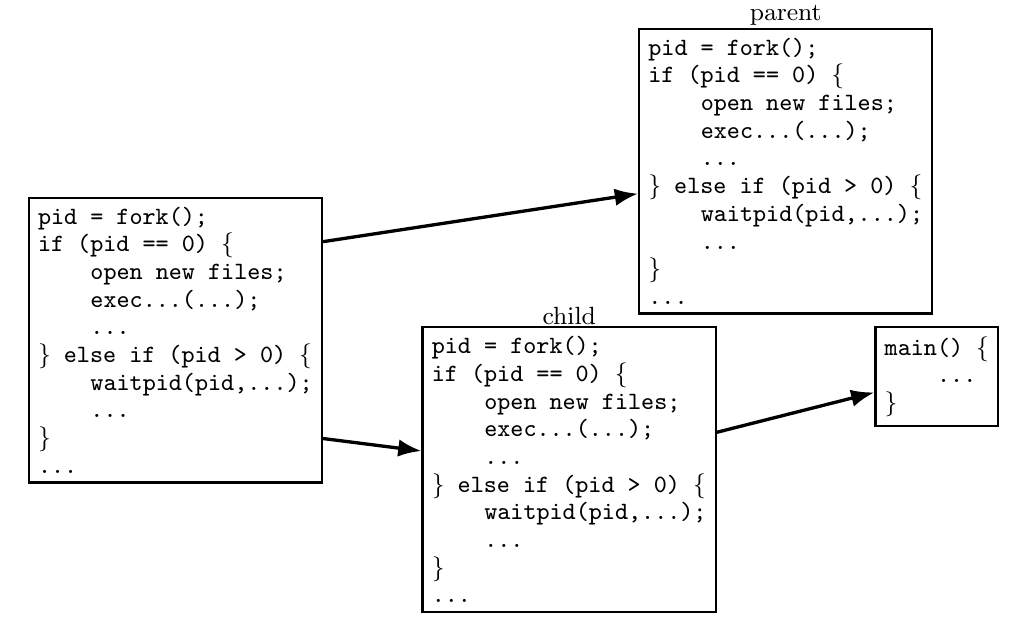
\begin{tikzpicture}
\tikzset{
    code box/.style={draw,thick,font=\tt\fontsize{9}{10}\selectfont,align=left},
    with the code/.style={
        code box,
    },
    with the other code/.style={
        code box,
    }
}
\node[with the code] (start) {\maincodeFork};
\node[with the code,anchor=south west,
      label={[font=\small,label distance=-1mm,overlay]north:parent}] (parent first) at ([xshift=4cm,yshift=-1.5cm]start.north east) {\maincodeWait};
\node[with the code,anchor=north west,
      label={[font=\small,label distance=-1mm]north:child}] (child first) at ([xshift=1.25cm,yshift=2cm]start.south east) {\maincodeOpenNew};
\node[with the other code,anchor=north west] (child second) at ([xshift=2cm]child first.north east) {\altcode};

\begin{scope}[very thick,>=Latex]
\draw[->] ([yshift=1.25cm]start.east) -- (parent first);
\draw[->] ([yshift=-1.25cm]start.east) -- (child first);
\draw[->] (child first) -- (child second);
\end{scope}
\end{tikzpicture}
\end{frame}

\begin{frame}{redirecting with exec}
\begin{itemize}
\item standard output/error/input are files
    \begin{itemize}
    \item (C stdout/stderr/stdin; C++ cout/cerr/cin)
    \end{itemize}
\vspace{.5cm}
\item (probably after forking) open files to redirect
\item \ldots and make them be standard output/error/input
    \begin{itemize}
    \item using \texttt{dup2()} library call
    \end{itemize}
\item then exec, preserving new standard output/etc.
\end{itemize}
\end{frame}


\subsection{dup2: redirection mechanism}

\begin{frame}<1>[fragile,label=reassign]{reassigning file descriptors}
\begin{itemize}
\item redirection: \verb|./program >output.txt|
\item step 1: open output.txt for writing, get new file descriptor
\item step 2: \myemph<2>{make that new file descriptor stdout (number 1)}
\vspace{.5cm}
\item<2-> tool: \texttt{int dup2(int oldfd, int newfd)} \\
        make \texttt{newfd} refer to same open file as \texttt{oldfd}
    \begin{itemize}
    \item same \textit{open file description}
    \item shares the current location in the file
    \item (even after more reads/writes)
    \end{itemize}
\item<2-> what if newfd already allocated --- closed, then reused
\end{itemize}
\end{frame}

\begin{frame}[fragile,label=dup2AndTable]{reassigning and file table}
\begin{lstlisting}[language=C,style=smaller]
// something like this in OS code
struct process_info { 
    ...
    struct open_file_description *files[SIZE];
    ....
};
...
process->files[STDOUT_FILENO] = process->files[opened-fd];
\end{lstlisting}
\begin{itemize}
\item syscall: \texttt{dup2(\textit{opened-fd}, STDOUT\_FILENO);}
\end{itemize}
\end{frame}

\againframe<2>{reassign}

\begin{frame}[fragile,label=dup2example]{dup2 example}
redirects stdout to output to \texttt{output.txt}:
\begin{lstlisting}[language=C++,style=small]
fflush(stdout);  /* clear printf's buffer */
int fd = open("output.txt",
              O_WRONLY | O_CREAT | O_TRUNC);
if (fd < 0)
    do_something_about_error();

dup2(fd, STDOUT_FILENO);
/* now both write(fd, ...) and write(STDOUT_FILENO, ...) 
   write to output.txt
   */

close(fd); /* only close original, copy still works! */

printf("This will be sent to output.txt.\n");
\end{lstlisting}
\end{frame}


\subsection{open/close/dup/fork and fd array}

\begin{frame}[fragile,label=openCloseAndFdArray]{open/dup/close/etc. and fd array}
\begin{lstlisting}[
    language=C++,
    moredelim={**[is][\btHL<1-|handout:1->]{@1}{1@}},
    style=smaller
]
// something like this in OS code
struct process_info {
  ...
  @1struct open_file_description *files[NUM];1@  
};
\end{lstlisting}
\begin{itemize}
\item open: \lstinline|files[new_fd] = ...;|
\item dup2(from, to): \lstinline|files[to] = files[from];|
\item close: \lstinline|files[fd] = NULL;|
\item fork: 
\begin{lstlisting}
  for (int i = ...)
      child->files[i] = parent->files[i];
\end{lstlisting}
\vspace{.25cm}
\item (plus extra work to avoid leaking memory)
\end{itemize}
\end{frame}


\subsection{exercise (read/write/dup2)}

\begin{frame}[fragile,label=ex]{exercise}
\begin{lstlisting}[style=small]
int fd = open("output.txt", O_WRONLY|O_CREAT|O_TRUNC, 0666);
write(fd, "A", 1);
dup2(STDOUT_FILENO, 100);
dup2(fd, STDOUT_FILENO);
write(STDOUT_FILENO, "B", 1);
write(fd, "C", 1);
close(fd);
write(STDOUT_FILENO, "D", 1);
write(100, "E", 1);
\end{lstlisting}
\small Assume \texttt{open()} and \texttt{dup2()} \textit{do not fail},
\texttt{write()} does not fail as long as the fd it writes to is open,
fd \texttt{100} was closed and is not what open returns, and \texttt{STDOUT\_FILENO} is initially open.
What is written to \texttt{output.txt}? \\
\begin{tabular}{llllll}
\textbf{A.} & ABCDE & \textbf{C.} & ABC & \textbf{E.} something else \\
\textbf{B.} & ABCD & \textbf{D.} & ACD \\
\end{tabular}
\end{frame}


\section{pipelines}

\subsection{pipe}

\begin{frame}{pipes}
\begin{itemize}
\item special kind of file: pipes
\item bytes go in one end, come out the other --- once
\vspace{.5cm}
\item created with \texttt{pipe()} library call
\item intended use: communicate between processes
    \begin{itemize}
    \item like implementing shell pipelines
    \end{itemize}
\end{itemize}
\end{frame}

\begin{frame}[fragile,label=pipe]{pipe()}
\begin{lstlisting}[language=C++,style=small]
int pipe_fd[2];
if (pipe(pipe_fd) < 0)
    handle_error();
/* normal case: */
int read_fd = pipe_fd[0];
int write_fd = pipe_fd[1];
\end{lstlisting}
then from one process\ldots
\begin{lstlisting}[language=C++,style=small]
write(write_fd, ...);
\end{lstlisting}
and from another
\begin{lstlisting}[language=C++,style=small]
read(read_fd, ...);
\end{lstlisting}
\end{frame}

\begin{frame}[fragile,label=pipeAndBlocking]{pipe() and blocking}
\myemph{BROKEN} example:
\begin{lstlisting}[language=C++,style=small]
int pipe_fd[2];
if (pipe(pipe_fd) < 0)
    handle_error();
int read_fd = pipe_fd[0];
int write_fd = pipe_fd[1];
write(write_fd, some_buffer, some_big_size);
read(read_fd, some_buffer, some_big_size);
\end{lstlisting}
This is likely to \myemph{not terminate}. What's the problem?
\end{frame}

\begin{frame}[fragile,label=pipeExample]{pipe example (1)}
\begin{lstlisting}[
    language=C++,
    style=smaller,
    moredelim={**[is][\btHL<2|handout:0>]{@2}{2@}},
    moredelim={**[is][\btHL<3|handout:2>]{@3}{3@}},
    moredelim={**[is][\btHL<4|handout:3>]{@4}{4@}},
]
int pipe_fd[2];
if (pipe(pipe_fd) < 0)
    handle_error(); /* e.g. out of file descriptors */
int read_fd = pipe_fd[0];
int write_fd = pipe_fd[1];
@2child_pid = fork();2@
@2if (child_pid  == 0) {2@
    /* in child process, write to pipe */
    @4close(read_fd);4@
    write_to_pipe(write_fd); /* function not shown */
    exit(EXIT_SUCCESS);
@2} else if (child_pid > 0) {2@
    /* in parent process, read from pipe */
    @3close(write_fd);3@
    read_from_pipe(read_fd); /* function not shown */
    @2waitpid(child_pid, NULL, 0);2@
    @4close(read_fd);4@
} @2else {2@ /* fork error */ }
\end{lstlisting}
\begin{tikzpicture}[overlay,remember picture]
\coordinate (box place) at ([xshift=-1cm,yshift=-1cm]current page.north east);
\tikzset{
    box/.style={draw=red,thick,fill=white,anchor=north east,at={(box place)},align=left,font=\small},
}
\begin{visibleenv}<2|handout:0>
\node[box] {
    `standard' pattern with fork()
};
\end{visibleenv}
\begin{visibleenv}<3|handout:2>
\node[box] {
    read() will not indicate \\
    end-of-file if write fd is open  \\
    (any copy of it)
};
\end{visibleenv}
\begin{visibleenv}<4|handout:3>
\node[box] {
    have habit of closing \\
    to avoid `leaking' file descriptors \\
    you can run out
};
\end{visibleenv}
\end{tikzpicture}
\end{frame}



\begin{frame}[fragile,label=pipeAndBlocking]{pipe() and blocking}
\myemph{BROKEN} example:
\begin{lstlisting}[language=C++,style=small]
int pipe_fd[2];
if (pipe(pipe_fd) < 0)
    handle_error();
int read_fd = pipe_fd[0];
int write_fd = pipe_fd[1];
write(write_fd, some_buffer, some_big_size);
read(read_fd, some_buffer, some_big_size);
\end{lstlisting}
This is likely to \myemph{not terminate}. What's the problem?
\end{frame}


\subsection{pipe and pipelines}

\usetikzlibrary{decorations.pathmorphing}

\begin{frame}[fragile,label=pipeAndPipelines]{pipe and pipelines}
\begin{Verbatim}[frame=single,fontsize=\small]
ls -1 | grep foo
\end{Verbatim}
\begin{lstlisting}[language=C++,style=smaller]
pipe(pipe_fd);
ls_pid = fork();
if (ls_pid == 0) {
    dup2(pipe_fd[1], STDOUT_FILENO);
    close(pipe_fd[0]); close(pipe_fd[1]);
    char *argv[] = {"ls", "-1", NULL};
    execv("/bin/ls", argv);
}
grep_pid = fork();
if (grep_pid == 0) {
    dup2(pipe_fd[0], STDIN_FILENO);
    close(pipe_fd[0]); close(pipe_fd[1]);
    char *argv[] = {"grep", "foo", NULL};
    execv("/bin/grep", argv);
}
close(pipe_fd[0]); close(pipe_fd[1]);
/* wait for processes, etc. */
\end{lstlisting}
\end{frame}

\begin{frame}[fragile,label=pipeDiagram]{example execution}
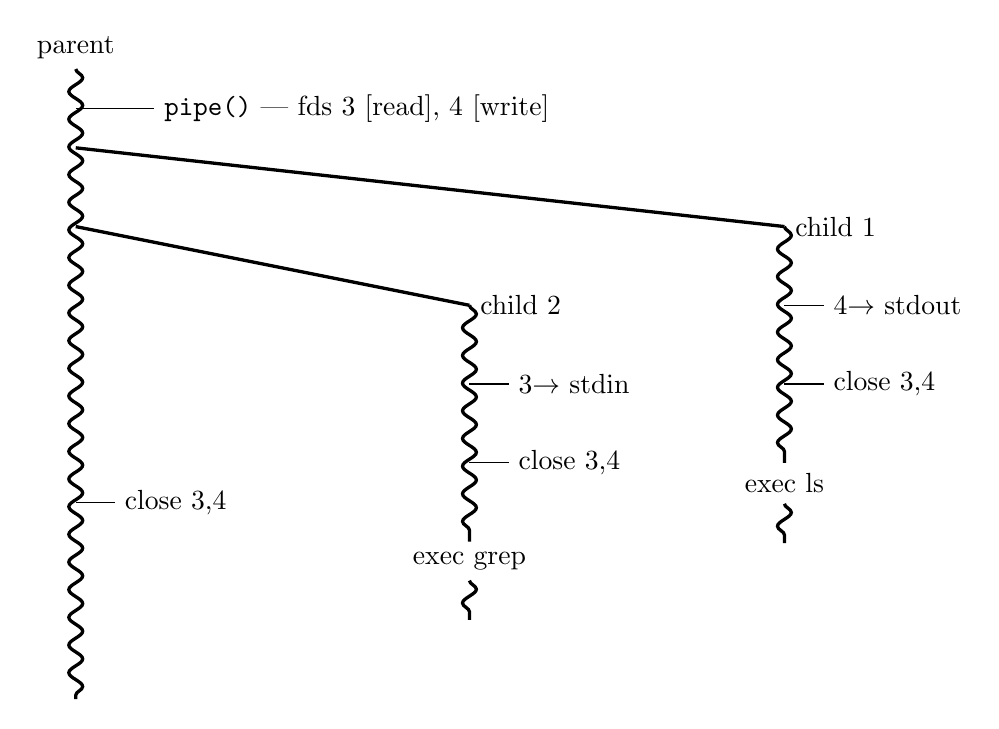
\begin{tikzpicture}
\tikzset{
    thread/.style={very thick,draw,decorate,decoration=snake},
    split/.style={very thick,draw},
    marker/.style={thin,draw},
}
\path[thread] (0, 0) --  (0, -8);
    \node[anchor=south] at (0,0) {parent};
\path[marker] (0, -.5) -- ++(1, 0) node[right] {\texttt{pipe()} --- fds 3 [read], 4 [write]};
    \path[split] (0, -1) --  (9, -2) node[right] {child 1};
    \path[marker] (9, -3) -- ++(.5, 0) node[right] {4$\rightarrow$ stdout};
    \path[marker] (9, -4) -- ++(.5, 0) node[right] {close 3,4};
    \path[thread] (9, -2) -- (9, -5) node[below] (exec ls) {exec ls};
    \path[thread] (exec ls.south) -- ++(0, -.5cm);

    \path[split] (0, -2) --  (5, -3) node[right] {child 2};
    \path[marker] (5, -4) -- ++(.5, 0) node[right] {3$\rightarrow$ stdin};
    \path[marker] (5, -5) -- ++(.5, 0) node[right] {close 3,4};
    \path[thread] (5, -3) -- (5, -6) node[below] (exec grep) {exec grep};
    \path[thread] (exec grep.south) -- ++(0, -.5cm);
    \path[marker] (0, -5.5) -- ++(.5, 0) node[right] {close 3,4};
\end{tikzpicture}
\end{frame}


% FIXME: better understanding that this works without write()/read() specifically?
